% Provenance (never printed): enseignement scientifique premiere (2019),
% "Le Soleil, notre source d'energie" (power received by latitude and
% season, albedo, the Earth's radiative balance, the small share stored by
% photosynthesis) and the old seconde/premiere S material on the
% atmosphere's energy; see sources/book2/PROVENANCE.md. Every insolation
% value, budget closure and photosynthesis figure is computed in
% figdata/grade-10/energy_budget.py; the budget fluxes are AR6 WG1
% Figure 7.2.
\chapter{The Earth's Energy Budget}\label{ch:g10:earth-energy-budget}

On the longest day of the year the Sun never sets at the North Pole. It
circles the sky all day at the same height, about \qty{23}{\degree} above
the horizon, and the top of the atmosphere above the pole receives in one
day more sunlight per square metre than anywhere else on the Earth ---
\qty{13.0}{kWh}, against \qty{9.5}{kWh} above the equator. Yet the sea
around the pole stays covered with ice through the summer. Over a whole
year, on the other hand, the equator receives two and a half times as much
sunlight as the pole, and the tropics stay warm all year round. This chapter
follows the energy of sunlight: how much arrives, where and when; how much is
reflected straight back to space; how the rest is shared between the air and
the ground, carried from the tropics towards the poles, and finally sent back
to space as infrared light --- and what tiny part of it ends up stored by
living things.
% ledger: earth:TSI, earth:obliquity (daily totals computed in figdata/grade-10/energy_budget.py)

\begin{omfigure}
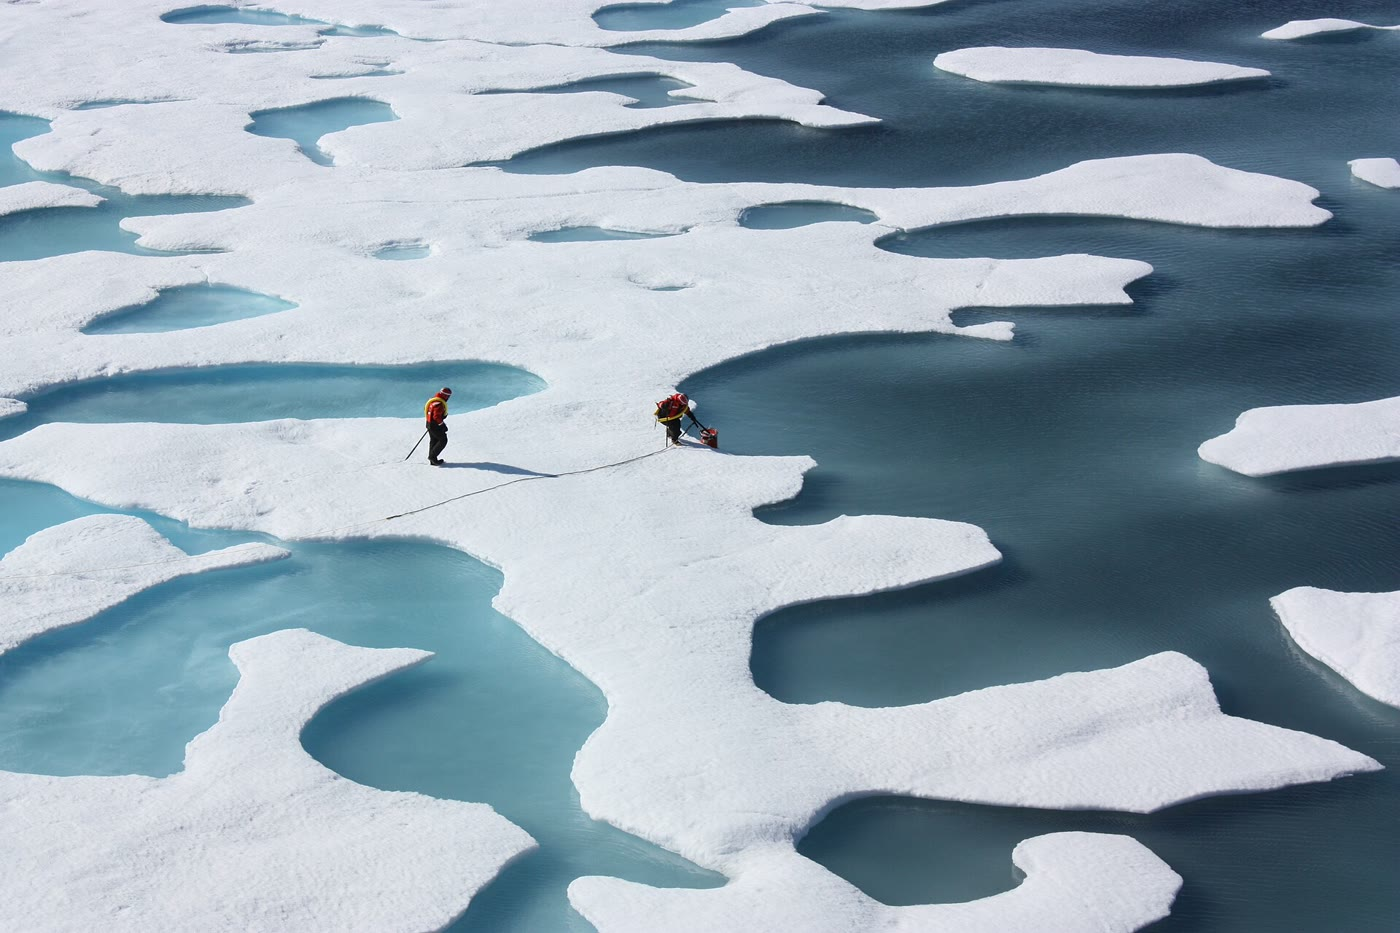
\includegraphics[width=0.78\linewidth]{images/book2/g10-nasa-melt-ponds.jpg}

{\small Sea ice in the Arctic Ocean in July, under a Sun that does not set:
white ice, pools of meltwater on its surface, and the dark open sea between
the floes. Two scientists sample the ponds. Photograph: NASA Goddard
Space Flight Center, 2011 (public domain).}
\end{omfigure}

\begin{recall}
The seasons come from the tilt of the Earth's axis, \qty{23.44}{\degree}
from the perpendicular to the plane of its orbit: in June the Northern
Hemisphere leans towards the Sun, which climbs higher in its sky and stays
up longer (the physics books, and Book 1). The irradiance at the Earth's
distance, $S_0 = \qty{1361}{W/m^2}$, the Bond \omterm{def:g10:earth-energy-budget:albedo}{albedo} of a planet and its
\omterm{def:g10:habitable-planet:equilibrium-temperature}{equilibrium temperature} were met in \cref{ch:g10:habitable-planet}.
Greenhouse gases absorb part of the infrared emitted by the surface (the
chemistry books). Warm air rises and cold air sinks, which sets the air
turning in convection cells and drives the global winds (Book 1, grade 8).
Plants, algae and some bacteria make sugars from carbon dioxide and water
with the energy of light: photosynthesis (the biology books).
\end{recall}

\section{Sunlight received}

Seen from the Sun, the Earth is a disc. Every second, it intercepts the
sunlight falling on a disc of radius $R$, its own radius; but that light is
shared among all the points of a sphere, half of which are in the night.

\begin{proposition}[A quarter of the solar constant]\label{prop:g10:earth-energy-budget:quarter}
Averaged over the whole surface of the Earth and over day and night, the
power of sunlight arriving at the top of the atmosphere is
\[
  \frac{S_0}{4} = \frac{1361}{4} \approx \qty{340}{W/m^2}.
\]
\end{proposition}

\begin{proof}
The Earth intercepts the sunlight crossing a disc of area $\pi R^2$
perpendicular to the rays, that is a power $S_0\,\pi R^2$. Spread over the
area of the sphere, $4\pi R^2$, this gives $S_0\,\pi R^2/(4\pi R^2) =
S_0/4$ per square metre.
\end{proof}
% ledger: earth:TSI, ipcc:budget-toa

\begin{omfigure}
\begin{tikzpicture}[font=\small, >={Stealth[length=2mm]}]
  \foreach \y in {-1.2,-0.8,...,1.21}
    \draw[->, omProp!80!black] (-3.4,\y) -- (-1.75,\y);
  \node[anchor=south, font=\footnotesize, align=center] at (-2.6,1.35) {sunlight,\\$S_0$ per m$^2$};
  \draw[fill=omProp!15, draw=omProp!80!black] (-1.6,0) ellipse (0.18 and 1.3);
  \node[anchor=north, font=\footnotesize, align=center] at (-1.6,-1.4) {disc\\$\pi R^2$};
  \shade[ball color=omDef!35] (1.2,0) circle (1.3);
  \fill[black, opacity=0.35] (1.2,1.3) arc (90:-90:1.3) arc (-90:90:0.35 and 1.3);
  \draw[omDef!80!black] (1.2,0) circle (1.3);
  \draw[dashed, black!50] (1.2,-1.3) arc (-90:90:0.35 and 1.3);
  \draw[<->] (1.2,0) -- node[above, font=\footnotesize] {$R$} (2.5,0);
  \node[anchor=west, font=\footnotesize, align=left] at (2.8,0.7) {sphere $4\pi R^2$:\\half in daylight,\\half in the night};
  \node[anchor=west, font=\footnotesize, align=left] at (2.8,-0.75) {average:\\$S_0\pi R^2/4\pi R^2 = S_0/4$};
\end{tikzpicture}

{\small The Earth intercepts the sunlight that falls on a disc of its own
radius, but shares it among the four-times larger area of a sphere: on
average, each square metre of the top of the atmosphere receives a quarter of
the solar constant.}
\end{omfigure}

The average hides great differences from place to place. A beam of sunlight
that strikes the ground at a slant spreads over a larger area than a beam
striking it straight on.

\begin{proposition}[Sunlight on a horizontal surface]\label{prop:g10:earth-energy-budget:height}
When the Sun is at a height $h$ above the horizon, a horizontal square metre
at the top of the atmosphere receives the power $S_0 \sin h$.
\end{proposition}

\begin{proof}
Take a beam of sunlight of cross-section \qty{1}{m^2}, square, carrying
$S_0$. On the ground its trace is a rectangle with one side of \qty{1}{m}
and the other of length $\ell$ along the slope of the rays. In the right
triangle formed by that side, the ray and the beam's cross-section, the
angle at the ground is $h$ and $\sin h = 1/\ell$. The beam's power is
spread over $\ell$ square metres: $S_0/\ell = S_0 \sin h$ per square
metre.
\end{proof}

\begin{omfigure}
\begin{tikzpicture}[font=\small, >={Stealth[length=2mm]}]
  \fill[omExo!15] (-0.3,-0.5) rectangle (6.3,0);
  \draw[thick] (-0.3,0) -- (6.3,0);
  \foreach \s in {0,0.3,...,1.21}
    \draw[->, omProp!80!black] ({0.6+\s/sin(35)+3.2*cos(35)},{3.2*sin(35)}) -- ({0.6+\s/sin(35)+0.02*cos(35)},{0.02*sin(35)});
  \draw[omProp!80!black, thick] (0.6,0) -- ({0.6+1.2/sin(35)},0);
  \draw (0.6,0) ++(1.6,0) arc (0:35:1.6);
  \node[font=\footnotesize] at ({0.6+1.85*cos(17)},{1.85*sin(17)}) {$h$};
  \draw[<->] (0.6,-0.25) -- node[below, font=\footnotesize] {$\ell = 1/\sin h$} ({0.6+1.2/sin(35)},-0.25);
  \node[anchor=south west, font=\footnotesize, align=left] at (4.35,1.95) {beam of\\cross-section\\\qty{1}{m^2}};
\end{tikzpicture}

{\small Sunlight arriving at a height $h$ above the horizon: the same beam
covers $1/\sin h$ square metres of horizontal ground, so each square metre
receives $S_0 \sin h$. The lower the Sun, the weaker the sunlight on the
ground.}
\end{omfigure}

The height of the Sun changes through the day, and the length of the day
changes with the seasons; both count in the energy a place receives.

\begin{definition}[Insolation]\label{def:g10:earth-energy-budget:insolation}
The \emph{insolation}\index{insolation} of a place is the power of sunlight
received by a horizontal square metre at the top of the atmosphere above
it. Averaged over the twenty-four hours of a day, it is the \emph{daily-mean
insolation}; averaged over a year, the \emph{annual-mean insolation}; both
are measured in \unit{W/m^2}.
\end{definition}

Working out the daily mean needs the Sun's height at every moment of the day,
which uses mathematics beyond this book; the computer that drew the
curves below did it. Two cases are simple. On
the equator at an equinox, the Sun rises due east, passes overhead at noon
and sets due west after twelve hours; averaged over twenty-four hours this
gives $S_0/\pi \approx \qty{433}{W/m^2}$ (admitted). At the North Pole the
Sun simply circles the sky at a constant height, which the next example
uses.

\begin{example}[The pole in June]\label{ex:g10:earth-energy-budget:pole}
% ledger: earth:TSI, earth:obliquity (values computed in figdata/grade-10/energy_budget.py)
At the June solstice the Sun stands \qty{23.44}{\degree} above the horizon
of the North Pole all day long. The daily-mean \omterm{def:g10:earth-energy-budget:insolation}{insolation} there is $1361
\times \sin 23.44^\circ \approx \qty{541}{W/m^2}$; over twenty-four hours
this is $541 \times 24 \approx \qty{13000}{Wh}$, \qty{13.0}{kWh} per square
metre. On the same day the equator receives a daily mean of
\qty{397}{W/m^2}, or \qty{9.5}{kWh} per square metre: the Sun rises higher
there at noon, but it is down for twelve hours.
\end{example}

\begin{omfigure}
\begin{tikzpicture}
\begin{axis}[omrecord, width=0.92\linewidth, height=6.4cm, xmin=1, xmax=365,
  ymin=0, ymax=600, ylabel={daily-mean insolation (\unit{W/m^2})},
  xtick={1,32,60,91,121,152,182,213,244,274,305,335},
  xticklabels={J,F,M,A,M,J,J,A,S,O,N,D}, xlabel={month},
  legend style={at={(0.5,1.02)}, anchor=south, legend columns=4, font=\footnotesize, draw=none},
  tick label style={font=\small}, label style={font=\small}]
\addplot[omThm!85!black, thick] table[x=day, y=Q0] {figdata/out/grade-10-energy_budget-daily.dat};
\addlegendentry{equator}
\addplot[omProp!90!black, thick, densely dashed] table[x=day, y=Q30] {figdata/out/grade-10-energy_budget-daily.dat};
\addlegendentry{\qty{30}{\degree} N}
\addplot[omMeth!85!black, thick, dashdotted] table[x=day, y=Q60] {figdata/out/grade-10-energy_budget-daily.dat};
\addlegendentry{\qty{60}{\degree} N}
\addplot[omDef!85!black, thick] table[x=day, y=Q90] {figdata/out/grade-10-energy_budget-daily.dat};
\addlegendentry{North Pole}
\end{axis}
\end{tikzpicture}

{\small Daily-mean \omterm{def:g10:earth-energy-budget:insolation}{insolation} at the top of the atmosphere through the year
at four latitudes of the Northern Hemisphere (computed for a circular orbit,
from the solar constant and the tilt of the axis). The pole receives nothing
for half the year and more than any other place around the June solstice.}
\end{omfigure}

\begin{remark}[Reading the curves]\label{rem:g10:earth-energy-budget:curves}
The equator's \omterm{def:g10:earth-energy-budget:insolation}{insolation} hardly changes: two shallow maxima at the
equinoxes, when the Sun passes overhead at noon. The farther north, the
larger the swing between summer and winter. Poleward of
$90^\circ - 23.44^\circ = \qty{66.56}{\degree}$ the Sun stays below the
horizon on the December solstice: the polar night. From about 10 May to the end
of July the North Pole and the latitude \qty{60}{\degree} N both receive more
than the equator.
\end{remark}

Over a whole year the picture changes: the annual-mean \omterm{def:g10:earth-energy-budget:insolation}{insolation}, plotted
in the section on surplus and deficit below, falls from \qty{416}{W/m^2} at the equator to \qty{172}{W/m^2} at
the poles. The summer abundance of the polar regions does not make up for
their long night and their low Sun.

\begin{remark}[The distance to the Sun does not make the seasons]\label{rem:g10:earth-energy-budget:distance}
% ledger: earth:peri, earth:aph, nasa:earth-perihelion-longitude (ratios computed)
The Earth's orbit is not quite a circle: its distance to the Sun varies
between \num{147.1} and \num{152.1} million kilometres, by about
\qty{3}{\percent}, so the sunlight varies by about \qty{7}{\percent}. The
Earth is closest to the Sun in early January, in the middle of the northern
winter. The curves above neglect this small change; the seasons come from
the tilt of the axis, and they are opposite in the two hemispheres.
\end{remark}

\section{Albedo}

Part of the sunlight reaching the Earth never warms anything: clouds, the air,
snow and the sea send it back to space.

\begin{definition}[Albedo]\label{def:g10:earth-energy-budget:albedo}
The \emph{albedo}\index{albedo} of a surface is the fraction of the sunlight
falling on it that it reflects, a number between 0 (all the light absorbed)
and 1 (all of it reflected). The Bond albedo of \cref{ch:g10:habitable-planet}
is the albedo of a planet taken as a whole.
\end{definition}

\begin{omfigure}
\begin{tikzpicture}[font=\small, x=9cm, y=0.55cm]
  \foreach \lab/\lo/\hi/\n in {fresh snow/0.80/0.90/8, sea ice/0.50/0.70/7,
      desert sand/0.40/0.40/6, whole Earth/0.30/0.30/5, green grass/0.25/0.25/4,
      bare soil/0.17/0.17/3, conifer forest/0.08/0.15/2, open ocean/0.06/0.06/1,
      fresh asphalt/0.04/0.04/0} {
    \fill[omDef!45] (0,\n-0.32) rectangle (\lo,\n+0.32);
    \ifdim\hi pt>\lo pt
      \fill[omDef!18] (\lo,\n-0.32) rectangle (\hi,\n+0.32);
      \draw[omDef!80!black] (\lo,\n-0.32) rectangle (\hi,\n+0.32);
    \fi
    \draw[omDef!80!black] (0,\n-0.32) rectangle (\lo,\n+0.32);
    \node[anchor=east, font=\footnotesize] at (-0.01,\n) {\lab};
  }
  \draw (0,-0.6) -- (1,-0.6);
  \foreach \x in {0,0.2,...,1.01}
    \draw (\x,-0.6) -- (\x,-0.75) node[below, font=\footnotesize] {\pgfmathprintnumber[fixed, precision=1]{\x}};
  \node[font=\footnotesize] at (0.5,-2.0) {albedo};
\end{tikzpicture}

{\small Typical \omterm{def:g10:earth-energy-budget:albedo}{albedos} of surfaces and of the Earth as a whole; the pale
part of a bar is the usual range. Data: University of Colorado Boulder,
MOSAiC expedition; National Snow and Ice Data Center.}
\end{omfigure}
% ledger: albedo:surfaces, nsidc:albedo-ice

Fresh snow returns most of the light it receives, the open ocean almost none.
This is why the sea ice of the opening photograph keeps its cold through the
polar summer: the snow on top of it reflects up to nine-tenths of the
sunlight, while the dark water between the floes absorbs about 94 per cent of it.
When the ice melts, dark water replaces it and absorbs more sunlight, which
melts more ice: a reinforcing loop that \cref{ch:g12:climate-change} weighs
among the feedbacks of the climate.

\begin{omfigure}
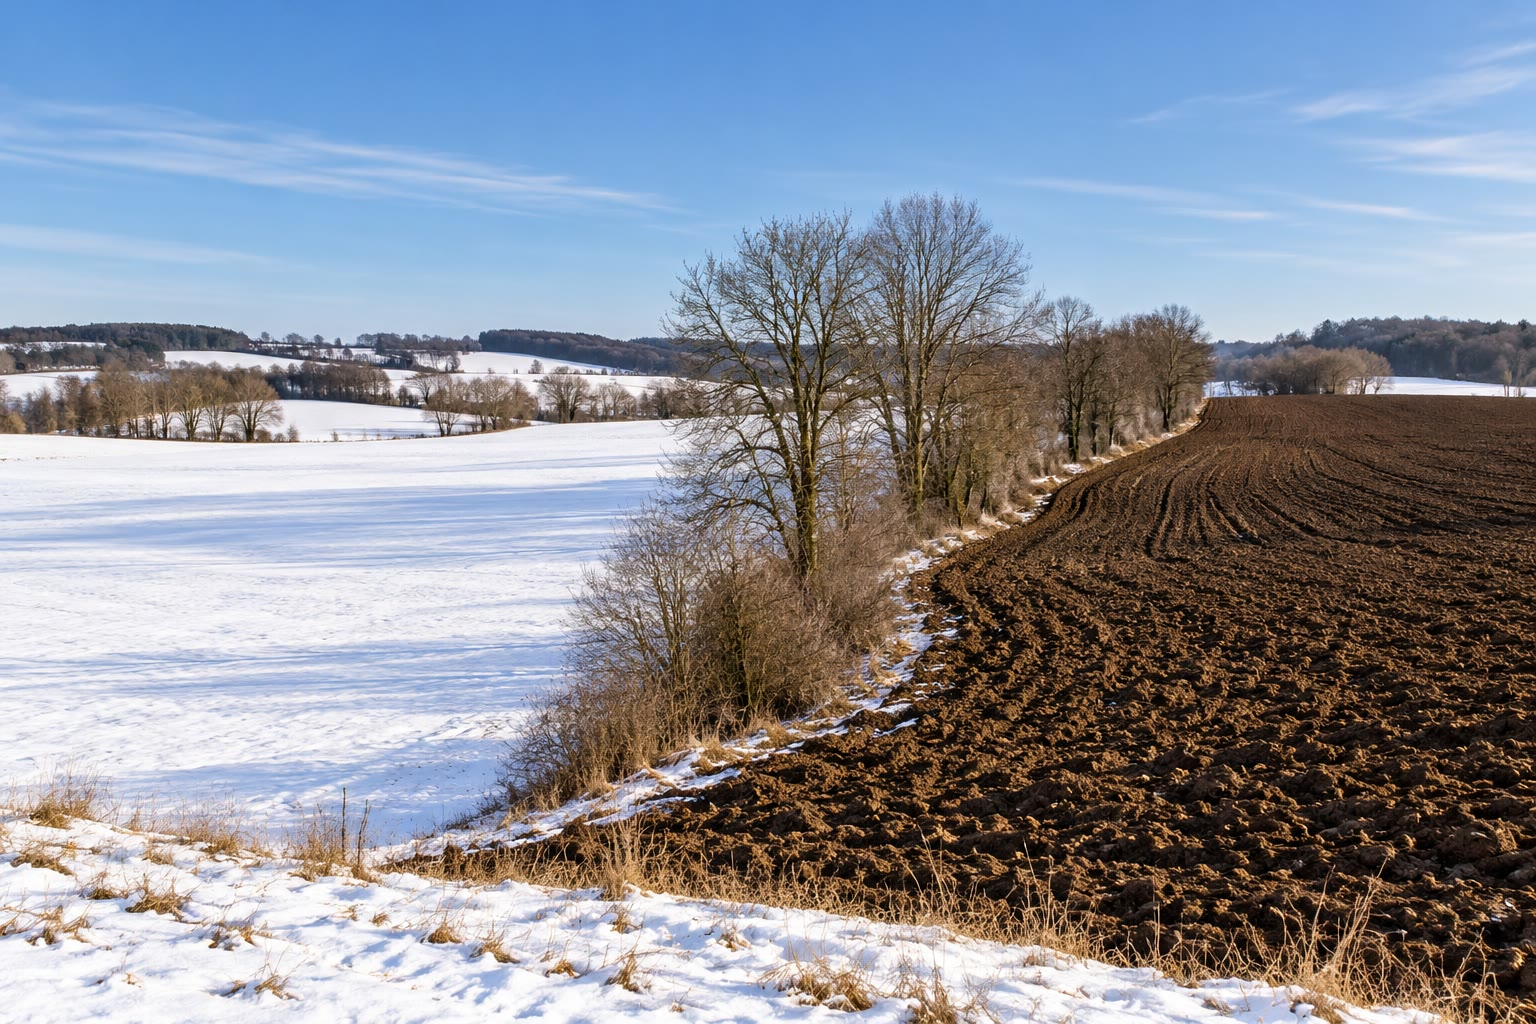
\includegraphics[width=0.7\linewidth]{images/book2/ai/g10-snow-and-ploughed-field.jpg}

{\small A winter morning after a few sunny days: the snow still lies on the
meadow, but it has melted on the dark ploughed field, which absorbs much
more of the sunlight.}
\end{omfigure}

For the Earth as a whole, the satellites measure the sunlight reflected to
space directly: on average \qty{100}{W/m^2} of the \qty{340}{W/m^2} that
arrive, an \omterm{def:g10:earth-energy-budget:albedo}{albedo} of $100/340 \approx 0.29$. Clouds are the main reflector:
the same measurements, with the clouds removed by calculation, give only
\qty{53}{W/m^2} reflected.
% ledger: ipcc:budget-toa, ipcc:budget-clearsky, earth:albedo

\begin{example}[The sunlight the Earth absorbs]\label{ex:g10:earth-energy-budget:absorbed}
% ledger: earth:TSI, earth:albedo, earth:Rmean (computed in figdata/grade-10/energy_budget.py)
With a Bond \omterm{def:g10:earth-energy-budget:albedo}{albedo} of 0.294, each square metre absorbs on average $340
\times (1 - 0.294) \approx \qty{240}{W/m^2}$. Over the whole sphere, of area
$4\pi R^2 = 4\pi \times (\qty{6.371e6}{m})^2 \approx \qty{5.10e14}{m^2}$, the
Earth absorbs $240 \times 5.10\times10^{14} \approx \qty{1.22e17}{W}$ of
sunlight: this power drives the winds, the ocean currents and the water
cycle.
\end{example}

\section{The global energy budget}

Where do these \qty{240}{W/m^2} go? Measurements from satellites, from
instruments on the ground and from ships, combined with models of the
atmosphere, now give a consistent answer, averaged over the globe and over
several years. The scientific assessment of 2021 summarises it in the
diagram below, and states that the global mean components are now known
more accurately, at the top of the atmosphere and at the surface (\emph{high
confidence}).
% ledger: ipcc:budget-confidence

\begin{definition}[Energy budget]\label{def:g10:earth-energy-budget:energy-budget}
The \emph{energy budget}\index{energy budget} of a system --- the whole
Earth, its surface or its atmosphere --- is the account of all the energy
entering and leaving it, each flow given as an average power per square
metre of the Earth's surface. The budget is \emph{balanced} when what enters
equals what leaves; otherwise the system gains or loses energy and warms or
cools.
\end{definition}

The surface also loses energy without any radiation: water evaporates from
the sea and from leaves, and the ground warms the air in contact with it.

\begin{definition}[Latent heat; sensible heat]\label{def:g10:earth-energy-budget:latent-heat}
The \emph{latent heat}\index{latent heat} of a substance is the energy it
absorbs when it changes state without changing temperature --- melting, or
evaporating --- and gives back when it changes back. For water evaporating
at \qty{15}{\degreeCelsius} it is about \qty{2.47}{MJ} per kilogram. In the
\omterm{def:g10:earth-energy-budget:energy-budget}{energy budget}, the \emph{latent heat flux} is the energy that evaporation
takes from the surface and that the water vapour releases in the air where
it condenses into clouds. The \emph{sensible heat}\index{sensible heat} flux
is the energy that the surface passes to the air in contact with it,
warming it, and that rising air carries upwards.
\end{definition}
% ledger: nist:water-latent

\begin{omfigure}
\begin{tikzpicture}[font=\footnotesize, >={Stealth[length=2.2mm, width=2mm]}, line width=1.4pt]
  % layers
  \fill[omDef!8] (0,0.5) rectangle (12.8,4.5);
  \fill[omExo!35] (0,0) rectangle (12.8,0.5);
  \draw[thin, black!60] (0,0.5) -- (12.8,0.5);
  \draw[thin, black!60, dashed] (0,4.5) -- (12.8,4.5);
  \node[anchor=east, black!70, align=right] at (-0.1,5.4) {space};
  \node[anchor=east, black!70, align=right] at (-0.1,4.5) {top of the\\atmosphere};
  \node[anchor=east, black!70, align=right] at (-0.1,2.5) {atmosphere};
  \node[anchor=east, black!70, align=right] at (-0.1,0.25) {surface};
  \pic[scale=0.7, transform shape] at (4.3,3.0) {puffycloud};
  \pic[scale=0.7, transform shape] at (6.2,3.0) {puffycloud};
  % sunlight
  \draw[->, omProp!90!black] (1.0,6.1) -- (1.0,0.52);
  \draw[->, omProp!90!black] (1.0,3.0) -- (1.6,3.0);
  \node[anchor=west, align=left] at (1.65,3.0) {80 absorbed\\by the air};
  \node[anchor=west] at (1.05,1.3) {185};
  \draw[->, omProp!55] (4.3,3.7) -- (4.3,6.1);
  \node[anchor=east] at (4.25,5.0) {75};
  \draw[->, omProp!55] (5.25,0.52) -- (5.25,6.1);
  \node[anchor=west] at (5.3,1.2) {25};
  % heat
  \draw[->, omMeth!80!black] (6.2,0.52) -- (6.2,2.95);
  \draw[->, omMeth!80!black] (7.8,0.52) -- (7.8,2.0);
  % infrared
  \draw[->, omThm!80!black] (9.2,0.52) -- (9.2,4.0);
  \draw[->, omThm!80!black] (10.7,3.4) -- (10.7,6.1);
  \draw[->, omThm!50] (12.1,4.0) -- (12.1,0.52);
  % words above the top of the atmosphere
  \node[anchor=south, align=center] at (1.0,6.15) {340\\incoming};
  \node[anchor=south, align=center] at (4.78,6.15) {100\\reflected};
  \node[anchor=south, align=center] at (7.7,5.0) {imbalance\\$+0.7$ absorbed};
  \node[anchor=south, align=center] at (10.7,6.15) {239 infrared\\to space};
  % words below the surface
  \node[anchor=north, align=center] at (1.0,-0.05) {160\\absorbed};
  \node[anchor=north, align=center] at (6.2,-0.05) {82\\latent\\heat};
  \node[anchor=north, align=center] at (7.8,-0.05) {21\\sensible\\heat};
  \node[anchor=north, align=center] at (9.4,-0.05) {398\\emitted};
  \node[anchor=north, align=center] at (12.1,-0.05) {342\\back\\radiation};
\end{tikzpicture}

{\small The global mean \omterm{def:g10:earth-energy-budget:energy-budget}{energy budget} of the Earth at the beginning of the
21st century, in \unit{W/m^2} averaged over the whole surface. Orange:
sunlight; green: heat carried by evaporation and by warm air; red: infrared.
Of the 100 reflected, 25 come from the surface and 75 from clouds, the air
and its dust. The infrared to space includes the part of the surface's
emission that escapes straight through the air. Data: IPCC, Sixth Assessment
Report, Working Group~I, Figure~7.2.}
\end{omfigure}
% ledger: ipcc:budget-toa, ipcc:budget-surface

\begin{method}[Reading an energy-budget diagram]\label{met:g10:earth-energy-budget:reading}
\begin{enumerate}
  \item Choose the system: the whole Earth (a line above the atmosphere),
        the surface, or the atmosphere (the layer between them).
  \item List the arrows that enter it and add them; list the arrows that
        leave it and add them.
  \item Compare the two sums. If they are equal within the rounding of the
        numbers, the system is in balance; the difference is what it gains
        (or loses) each second per square metre.
\end{enumerate}
\end{method}

\begin{proposition}[The budget balances]\label{prop:g10:earth-energy-budget:balance}
Within the rounding of the figures, the budget in the diagram
above is balanced for the Earth as a
whole, for the surface and for the atmosphere, apart from a small surplus of
about \qty{0.7}{W/m^2} that the Earth absorbs and does not give back.
\end{proposition}

\begin{proof}
\emph{Whole Earth:} in, 340; out, $100 + 239 = 339$. \emph{Surface:} in,
$160 + 342 = 502$; out, $82 + 21 + 398 = 501$. In both cases the surplus,
about 1, is the imbalance of 0.7 rounded. \emph{Atmosphere:} call $W$ the
part of the surface's infrared that escapes through the air to space. The air
receives $80 + 82 + 21 + (398 - W) = 581 - W$ and emits $342$ downwards and
$239 - W$ upwards, $581 - W$ in all: balanced, whatever $W$.
\end{proof}
% ledger: ipcc:budget-toa, ipcc:budget-surface (closures checked in figdata/grade-10/energy_budget.py)

The diagram also shows the greenhouse effect at work. The surface receives
from the air, as infrared, \qty{342}{W/m^2} --- more than twice the sunlight
it absorbs, \qty{160}{W/m^2}. This is why it can emit \qty{398}{W/m^2}, the
emission of a body at about \qty{15}{\degreeCelsius}, while the Earth sends
only \qty{239}{W/m^2} to space. The physics books build the model that
connects these numbers to the temperature; this book uses the measured
fluxes.

\begin{example}[A metre of water a year]\label{ex:g10:earth-energy-budget:evaporation}
% ledger: ipcc:budget-surface, nist:water-latent (computed in figdata/grade-10/energy_budget.py)
The \omterm{def:g10:earth-energy-budget:latent-heat}{latent heat} flux, \qty{82}{W/m^2}, evaporates every second $82/2.47\times
10^6 \approx \qty{3.3e-5}{kg}$ of water per square metre. Over a year,
$3.16\times10^7$ seconds, this makes about \qty{1050}{kg}, a layer of water
\qty{1.05}{m} thick over the whole Earth. The air holds only a little water
at a time, so practically all of it falls back as rain and snow: the \omterm{def:g10:earth-energy-budget:latent-heat}{latent
heat} flux and the yearly rainfall of the planet are two faces of the same
water cycle.
\end{example}

\begin{remark}[The imbalance]\label{rem:g10:earth-energy-budget:imbalance}
% ledger: ipcc:budget-toa, ipcc:heating
The surplus of \qty{0.7}{W/m^2} looks tiny next to the fluxes of hundreds of
watts, but over the whole Earth it is $0.7 \times 5.10\times10^{14} \approx
\qty{3.6e14}{W}$, mostly stored in the ocean, which warms. It is not a
natural constant: it has grown in recent decades, as
\cref{ch:g12:climate-change} explains.
\end{remark}

\section{Surplus and deficit}

The budget balances for the Earth as a whole, but not at each latitude.

\begin{omfigure}
\begin{tikzpicture}
\begin{axis}[omrecord, width=0.86\linewidth, height=5.6cm, xmin=0, xmax=90,
  ymin=0, ymax=450, xlabel={latitude (\unit{\degree})},
  ylabel={annual-mean insolation (\unit{W/m^2})}, xtick={0,15,...,90},
  tick label style={font=\small}, label style={font=\small}]
\addplot[omThm!85!black, thick] table[x=lat, y=Qann] {figdata/out/grade-10-energy_budget-annual.dat};
\addplot[omDef!80!black, dashed, domain=0:90] {340.25};
\node[anchor=south west, font=\footnotesize, omDef!80!black] at (axis cs:2,343) {global mean, 340};
\node[anchor=south west, font=\footnotesize, omThm!85!black] at (axis cs:62,232) {annual mean};
\end{axis}
\end{tikzpicture}

{\small Annual-mean \omterm{def:g10:earth-energy-budget:insolation}{insolation} at the top of the atmosphere against latitude
(the same in both hemispheres; computed from the solar constant and the tilt
of the axis). Between the equator and about \qty{37}{\degree} it exceeds the
global mean; poleward it falls short.}
\end{omfigure}

The tropics absorb far more sunlight than the polar regions, and their low
\omterm{def:g10:earth-energy-budget:albedo}{albedo} widens the gap. The infrared they send to space is larger too,
because they are warmer, but it varies much less with latitude. As a result,
the regions around the equator absorb on average about \qty{200}{W/m^2} more
than they reflect and radiate, and the regions near the poles radiate about
\qty{200}{W/m^2} more than they absorb.
% ledger: nasaeo:surplus

\begin{definition}[Poleward heat transport]\label{def:g10:earth-energy-budget:heat-transport}
The \emph{poleward heat transport}\index{poleward heat transport} is the
flow of energy carried from the tropics towards the poles by the motions of
the atmosphere and of the ocean. It is measured, across a circle of
latitude, in petawatts (\qty{1}{PW} = \qty{e15}{W}).
\end{definition}

Without it, the tropics would grow hotter and the poles colder until each
latitude balanced its own budget. The atmosphere does most of the carrying:
warm air moving poleward and cold air returning towards the equator, and
water vapour that releases its \omterm{def:g10:earth-energy-budget:latent-heat}{latent heat} far from where it evaporated. The
ocean currents carry the rest. Estimates from measurements put the
atmosphere's poleward transport at a maximum of about \qty{5.0}{PW} near
\qty{43}{\degree} N, with similar values near \qty{40}{\degree} S; the ocean
carries more than the atmosphere only close to the equator, between
\qty{0}{\degree} and \qty{17}{\degree} N, and at \qty{35}{\degree} N, where
the total transport is largest, the atmosphere carries \qty{78}{\percent} of
it. The total is largest there because \qty{35}{\degree} is about where the
surplus gives way to the deficit: equatorward, the transport keeps gathering
the surplus of every latitude it crosses; poleward, each latitude draws on
it.
% ledger: trenberth:transport

\begin{omfigure}
\begin{tikzpicture}[font=\footnotesize, >={Stealth[length=2mm]}]
  \def\R{2.4}
  \begin{scope}
    \clip (0,0) circle (\R);
    \fill[omThm!22] (-\R,{-\R*sin(35)}) rectangle (\R,{\R*sin(35)});
    \fill[omDef!22] (-\R,{\R*sin(35)}) rectangle (\R,\R);
    \fill[omDef!22] (-\R,-\R) rectangle (\R,{-\R*sin(35)});
  \end{scope}
  \draw[thick] (0,0) circle (\R);
  \draw[black!50] (-\R,0) -- (\R,0);
  \foreach \s in {1,-1} \draw[black!40, dashed] ({-\R*cos(35)},{\s*\R*sin(35)}) -- ({\R*cos(35)},{\s*\R*sin(35)});
  \node at (0,0.45) {surplus};
  \node at (0,1.95) {deficit};
  \node at (0,-1.95) {deficit};
  \node[anchor=west, black!60] at (\R+0.05,0) {equator};
  \node[anchor=west, black!60] at ({\R*cos(35)+0.05},{\R*sin(35)}) {\qty{35}{\degree} N};
  \node[anchor=west, black!60] at ({\R*cos(35)+0.05},{-\R*sin(35)}) {\qty{35}{\degree} S};
  \foreach \s in {1,-1} {
    \draw[->, very thick, omProp!90!black] ({-(\R+0.35)*cos(10)},{\s*(\R+0.35)*sin(10)}) arc ({180-10*\s}:{180-70*\s}:{\R+0.35});
    \draw[->, thick, omMeth!80!black] ({-(\R-0.45)*cos(8)},{\s*(\R-0.45)*sin(8)}) arc ({180-8*\s}:{180-55*\s}:{\R-0.45});
  }
  \node[anchor=east, omProp!90!black, align=right] at (-\R-0.75,1.6) {atmosphere};
  \node[anchor=east, omProp!90!black, align=right] at (-\R-0.75,-1.6) {atmosphere};
  \node[omMeth!80!black] at (-1.25,0.62) {ocean};
  \node[omMeth!80!black] at (-1.25,-0.62) {ocean};
\end{tikzpicture}

{\small Between about \qty{35}{\degree} S and \qty{35}{\degree} N the Earth
absorbs more energy than it radiates; poleward of these latitudes it
radiates more than it absorbs. The atmosphere (orange) and the ocean (green)
carry the surplus towards the poles. Schematic: the widths of the arrows are
not to scale.}
\end{omfigure}

This transport is the engine of the weather. The convection cells and the
global winds of Book 1, the storms of \cref{ch:g10:storms-and-cyclones} and
the great ocean currents of \cref{ch:g10:layered-ocean} all move heat from
where the Sun gives too much to where it gives too little.

\section{Where the energy goes}

Almost all the energy of sunlight that the Earth absorbs ends up as heat:
it warms the ground, the sea and the air, evaporates water, drives the
winds and the currents, and leaves again as infrared light. A tiny part takes
a different path: photosynthesis stores it in the chemical bonds of sugars,
and from there in all the living matter of the planet.

\begin{example}[The share of photosynthesis]\label{ex:g10:earth-energy-budget:photosynthesis}
% ledger: field:npp, nist:glucose-combustion, earth:Rmean (computed in figdata/grade-10/energy_budget.py)
Plants on land and algae in the sea store, after their own needs, about
\num{105} billion tonnes of carbon in new living matter each year, roughly
half on land and half in the ocean: ecologists call it the net primary
production of the planet. Burning a mole of glucose,
\ce{C6H12O6}, which contains six moles of carbon, \qty{72}{g}, releases
\qty{2805}{kJ}: about \qty{38.9}{kJ} per gram of carbon. The energy stored
each year is $1.049\times10^{17}\,\unit{g} \times \qty{38.9e3}{J/g} \approx
\qty{4.1e21}{J}$, a power of $4.1\times10^{21}/3.16\times10^{7} \approx
\qty{1.3e14}{W}$. Compared with the \qty{1.22e17}{W} of sunlight the Earth
absorbs, this is about \qty{0.1}{\percent}.
\end{example}

\begin{remark}[A small share, a large role]\label{rem:g10:earth-energy-budget:life}
One thousandth of the absorbed sunlight feeds nearly all life on the Earth,
and the remains of plants and algae buried over hundreds of millions of years
make up coal, oil and natural gas (\cref{ch:g11:fossil-fuel-geology}). The
rest of the sunlight --- more than 99.9 per cent --- keeps the planet warm
and its air, water and weather moving.
\end{remark}

\section{Exercises}

\begin{exercise}[$\star$]\label{exo:g10:earth-energy-budget:1}
Define the \omterm{def:g10:earth-energy-budget:insolation}{insolation} of a place and the \omterm{def:g10:earth-energy-budget:albedo}{albedo} of a surface. Which reflects
the larger fraction of sunlight, fresh snow or the open ocean?
\end{exercise}

\begin{exercise}[$\star$]\label{exo:g10:earth-energy-budget:2}
Using the energy-budget diagram of this chapter, give as percentages of the
\qty{340}{W/m^2} arriving at the top of the atmosphere the share reflected
to space, the share absorbed by the air and the share absorbed by the
surface.
\end{exercise}

\begin{exercise}[$\star$]\label{exo:g10:earth-energy-budget:3}
A summer sun delivers \qty{800}{W/m^2} to the ground. How much power does a
square metre absorb if it is covered with fresh asphalt (\omterm{def:g10:earth-energy-budget:albedo}{albedo} 0.04), and
with fresh snow (\omterm{def:g10:earth-energy-budget:albedo}{albedo} 0.85)?
\end{exercise}

\begin{exercise}[$\star$]\label{exo:g10:earth-energy-budget:4}
Which carries more energy away from the Earth's surface, evaporation or the
warming of the air in contact with the ground? Describe in two sentences how
the energy taken by evaporation from the sea reaches the air high above it.
\end{exercise}

\begin{exercise}[$\star$]\label{exo:g10:earth-energy-budget:5}
Explain why the daily-mean \omterm{def:g10:earth-energy-budget:insolation}{insolation} is zero at the North Pole in December,
and give the latitude beyond which this happens on the December solstice.
\end{exercise}

\begin{exercise}[$\star\star$]\label{exo:g10:earth-energy-budget:6}
Using \cref{prop:g10:earth-energy-budget:height}, compute the power received
by a horizontal square metre at the top of the atmosphere when the Sun is
\qty{90}{\degree}, \qty{30}{\degree} and \qty{10}{\degree} above the horizon.
At what height of the Sun does the square metre receive half of $S_0$?
\end{exercise}

\begin{exercise}[$\star\star$]\label{exo:g10:earth-energy-budget:7}
Following \cref{met:g10:earth-energy-budget:reading}, check the budget of
sunlight alone: of the \qty{340}{W/m^2} that arrive, how much is reflected,
absorbed by the air and absorbed by the surface? Do the three add up to 340?
Check also that the sunlight reaching the surface, \qty{185}{W/m^2}, is
either reflected or absorbed there.
\end{exercise}

\begin{exercise}[$\star\star$]\label{exo:g10:earth-energy-budget:8}
With the Earth's mean radius \qty{6371}{km}, compute the area of the disc
that intercepts sunlight and the power it intercepts, then the area of the
sphere. Deduce the average power per square metre of the sphere.
\end{exercise}

\begin{exercise}[$\star\star$]\label{exo:g10:earth-energy-budget:9}
The Earth's surplus is \qty{0.7}{W/m^2} over an area of
\qty{5.10e14}{m^2}. How much energy, in joules, does the Earth gain in a year
of $3.16\times10^7$ seconds?
\end{exercise}

\begin{exercise}[$\star\star$]\label{exo:g10:earth-energy-budget:10}
With the clouds removed by calculation, the Earth would reflect
\qty{53}{W/m^2} instead of \qty{100}{W/m^2}, and send \qty{267}{W/m^2} of
infrared to space instead of \qty{239}{W/m^2}. By how much do the clouds
change the sunlight absorbed, and the infrared lost? Do the clouds, on
balance, warm or cool the Earth?
\end{exercise}

\begin{exercise}[$\star\star$]\label{exo:g10:earth-energy-budget:11}
Read the curves of daily-mean \omterm{def:g10:earth-energy-budget:insolation}{insolation} in this chapter. In which months is the
daily-mean \omterm{def:g10:earth-energy-budget:insolation}{insolation} at the North Pole larger than at the equator? Why does
the equator's curve show two maxima and not one?
\end{exercise}

\begin{exercise}[$\star\star\star$]\label{exo:g10:earth-energy-budget:12}
The \omterm{def:g10:earth-energy-budget:latent-heat}{latent heat} of evaporation of water is \qty{2.47}{MJ/kg} and the \omterm{def:g10:earth-energy-budget:latent-heat}{latent
heat} flux \qty{82}{W/m^2}. Compute the thickness of water, in millimetres,
evaporated from the average square metre of the Earth each day, and in metres
each year (one litre of water spread over a square metre makes a layer
\qty{1}{mm} thick).
\end{exercise}

\begin{exercise}[$\star\star\star$]\label{exo:g10:earth-energy-budget:13}
At the North Pole the Sun circles the sky at a height equal to its
declination $\delta$, so the daily-mean \omterm{def:g10:earth-energy-budget:insolation}{insolation} there is $S_0 \sin
\delta$. Find the declination for which the pole receives as much, on
average over the day, as the equator at an equinox, $S_0/\pi$. The
declination obeys $\sin\delta = \sin 23.44^\circ \times \sin\lambda$, where
the angle $\lambda$ grows steadily by \qty{360}{\degree} in a year, from
\qty{0}{\degree} at the March equinox (\qty{90}{\degree} at the June
solstice). For roughly how many days a year does the pole receive more than
$S_0/\pi$?
\end{exercise}

\begin{exercise}[$\star\star\star$]\label{exo:g10:earth-energy-budget:14}
Suppose that in summer an area of \qty{1e12}{m^2} of sea ice (\omterm{def:g10:earth-energy-budget:albedo}{albedo} 0.6)
melts and is replaced by open ocean (\omterm{def:g10:earth-energy-budget:albedo}{albedo} 0.06), under sunlight of
\qty{300}{W/m^2} on average at the surface. Compute the extra power
absorbed. Compare it with the power stored by all the photosynthesis on
the Earth, \qty{1.3e14}{W}, and explain why this exchange of surfaces
reinforces itself.
\end{exercise}

\begin{exercise}[$\star\star\star$]\label{exo:g10:earth-energy-budget:15}
The Earth's distance to the Sun is \num{147.1} million kilometres at its
closest and \num{152.1} million at its farthest, for a mean of
\num{149.6} million, where $S_0 = \qty{1361}{W/m^2}$. Compute the solar
irradiance at the two extremes. The difference is close to
\qty{90}{W/m^2}; at \qty{60}{\degree} N, the daily-mean \omterm{def:g10:earth-energy-budget:insolation}{insolation} is about
\qty{490}{W/m^2} in June and \qty{24}{W/m^2} in December. Explain why the
distance cannot be the cause of the seasons.
\end{exercise}

\section{Problem: Following a Sunbeam}

\begin{problem}[{Weekend problem --- from the sunlight that reaches the Earth
to the share that life stores}]
\label{pb:g10:earth-energy-budget:1}
% ledger: earth:TSI, earth:Rmean, ipcc:budget-toa, ipcc:budget-surface, ipcc:budget-clearsky, nist:water-latent, field:npp, nist:glucose-combustion (all results computed in figdata/grade-10/energy_budget.py or from the rounded data below)
Use $S_0 = \qty{1361}{W/m^2}$, the Earth's radius $R = \qty{6371}{km}$,
$\sigma = \qty{5.67e-8}{W.m^{-2}.K^{-4}}$, a year of $3.156\times10^7$
seconds, the fluxes of the energy-budget diagram, a \omterm{def:g10:earth-energy-budget:latent-heat}{latent
heat} of evaporation of \qty{2.47}{MJ/kg}, a global net primary production of
\num{104.9} billion tonnes of carbon per year, and \qty{2805}{kJ} released
by burning a mole of glucose (\qty{72.07}{g} of carbon).

\medskip
\noindent\textbf{Part I --- The geometry of sunlight.}
\begin{enumerate}
  \item Compute the area of the disc that intercepts sunlight, $\pi R^2$, in
        square metres.
  \item Compute the power of sunlight it intercepts.
  \item Compute the area of the Earth's surface, $4\pi R^2$.
  \item Deduce the average power arriving per square metre of the top of the
        atmosphere.
  \item At an equinox at noon, the Sun is overhead on the equator and
        \qty{30}{\degree} above the horizon at \qty{60}{\degree} N. What does
        a horizontal square metre receive at each place?
\end{enumerate}

\medskip
\noindent\textbf{Part II --- Albedo.}
\begin{enumerate}[resume]
  \item From the \qty{100}{W/m^2} reflected, compute the Earth's \omterm{def:g10:earth-energy-budget:albedo}{albedo}.
  \item Compute the power absorbed per square metre and by the whole Earth.
  \item Without clouds, \qty{53}{W/m^2} would be reflected. What would the
        \omterm{def:g10:earth-energy-budget:albedo}{albedo} be? By what factor do clouds raise it?
  \item Compute the \omterm{def:g10:habitable-planet:equilibrium-temperature}{equilibrium temperature} corresponding to the absorbed
        power of question 7 (\cref{ch:g10:habitable-planet}), and compare it
        with the surface's \qty{288}{K}.
\end{enumerate}

\medskip
\noindent\textbf{Part III --- The surface.}
\begin{enumerate}[resume]
  \item Add the energy flows that enter the surface.
  \item Add those that leave it, and compare.
  \item How many times larger than the sunlight absorbed by the surface is
        the infrared it receives from the air? What does this show?
  \item Compute the mass of water evaporated from a square metre in a year,
        and the thickness of the layer it makes.
  \item Compute the total power of the imbalance, \qty{0.7}{W/m^2}, over the
        whole Earth.
\end{enumerate}

\medskip
\noindent\textbf{Part IV --- The share of life.}
\begin{enumerate}[resume]
  \item Compute the energy stored per gram of carbon fixed in glucose.
  \item Compute the energy stored in a year by the net primary production.
  \item Convert it into a power.
  \item Express it per square metre of the Earth's surface.
  \item Compare it with the imbalance of question 14.
  \item What share of the sunlight absorbed by the Earth (question 7) does
        photosynthesis store?
\end{enumerate}
\end{problem}
